\chapter{Einleitung}
Im Sommersemester 2016 begann an der Hochschule Karlsruhe im Rahmen eines Entwicklungsprojektes die Entwicklung eines balancierenden Würfels. Die Idee hierfür lieferte der Cubli \cite{Cubli1}, welcher an der ETH Zürich entworfen wurde. Die Aufgabe des Projekts bestand darin, einen Würfel mit einer Kantenlänge von $15\text{ cm}$ zu entwerfen, der in der Lage ist auf seinen Kanten und Ecken zu balancieren. Hierfür werden im Inneren des Würfels drei Motoren mit jeweils einer Schwungmasse montiert. Die Drehmomente der Motoren dienen als Stellgrößen eines Reglers, um den Würfel in einer aufrechten Position zu balancieren. Allerdings ist es nicht möglich mithilfe der Motormomente den Würfel aus einer beliebigen Position auf seine Kanten oder Ecken zu richten, da das maximale Motormoment das Gravitationsmoment nur in einem begrenzten Gebiet überwinden kann. Um dieses Problem zu lösen, werden die Schwungmassen als Energiespeicher verwendet. Die Schwungmassen werden zunächst beschleunigt und im Anschluss mittels einer mechanischen Bremse gestoppt, wodurch deren Drehimpuls auf das Würfelgehäuse übertragen wird und ein ausreichendes Drehmoment entsteht, um den Würfel aufzurichten.
\begin{figure}[!ht]
\centering
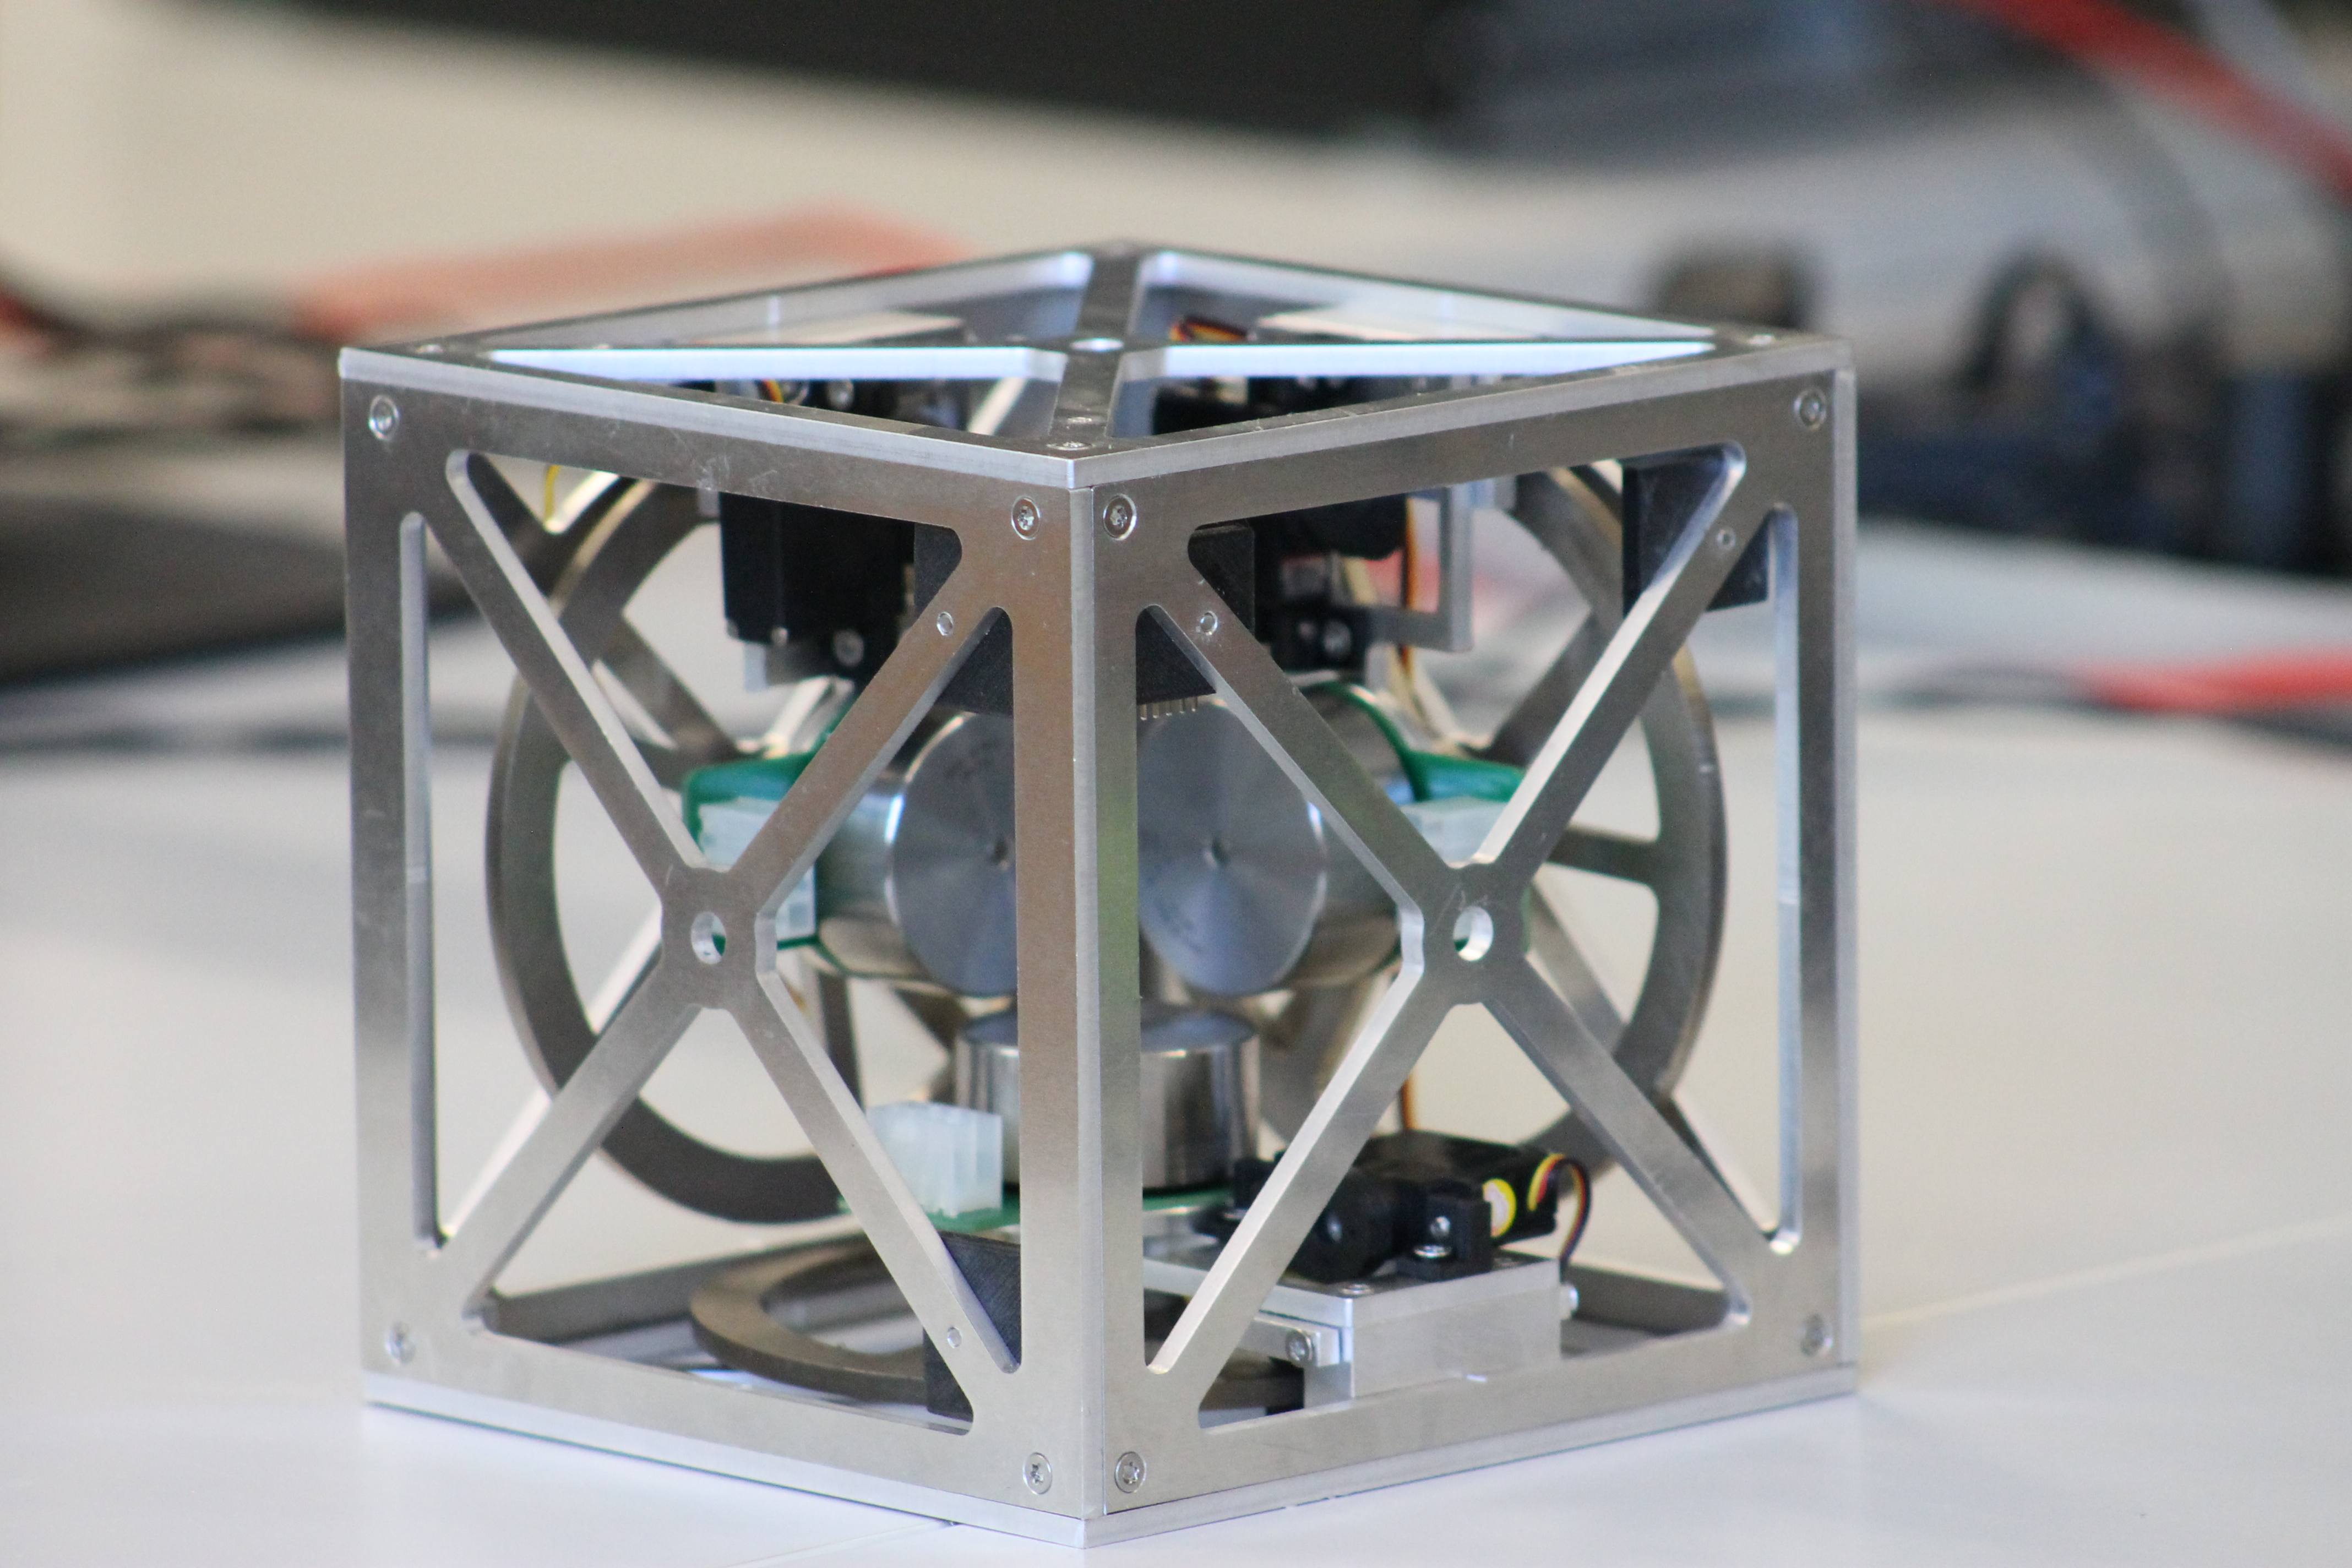
\includegraphics[width=0.85\linewidth]{img/3D_Modell_img.jpg}
\caption{Prototyp des Würfels}
\end{figure}


In dem vorangehenden Entwicklungsprojekt wurde zunächst eine einzelne Würfelseite mit einem Motor konzipiert. Dieses Modell lässt sich mit dem auf einer Kante balancierenden Würfel vergleichen. Die Bewegungsgleichungen der Würfelseite wurden mithilfe des Lagrange-Formalismus hergeleitet und anschließend für den Entwurf eines Zustandsreglers verwendet. Der Regler ermöglicht das Balancieren der Würfelseite in der aufrechten Position. Um die Zustandsgrößen zu messen, sind an der Würfelseite zwei Sensormodule montiert, welche deren Beschleunigung- und Winkelgeschwindigkeit entlang dreier Achsen erfassen. Hierbei werden die Beschleunigungswerte genutzt, um nach \cite{Cubli1} die Ausrichtung der Würfelseite zu bestimmen. Des Weiteren sind in dem Motor Hall-Sensoren integriert, um die Winkelgeschwindigkeit der Schwungmasse zu ermitteln. Für die Umsetzung des zeitdiskreten Reglers wird ein BeagleBone Black verwendet, auf welchem ein Linux-Betriebssystem ausgeführt wird. Der letzte Aufgabenteil des Entwicklungsprojektes bestand in der Konstruktion und Fertigung des Würfels.

Die Aufgabe dieser Arbeit besteht darin ein Konzept zu entwickeln, um den Würfel auf einer seiner Ecken zu balancieren. Hierunter fallen mehrere Teilaufgaben. Zunächst ist die Systemdynamik in Form eines mathematischen Modells zu erfassen. Anhand dieses Modells muss ein Regler entworfen werden, um den Würfel auf einer Ecke zu stabilisieren. Hierbei sind mögliche Ansätze der Regelungstechnik zu recherchieren und mittels einer Simulation zu vergleichen. Des Weiteren muss ein Konzept für die Erfassung der Zustandsgrößen, welche für die Regelung relevant sind, erarbeitet werden. Die letzte Teilaufgabe besteht darin, das Regelungskonzept mittels einer Embedded Plattform zu implementieren und an der Strecke zu erproben. Das Gesamtsystem wird anhand seiner Fähigkeit, den Würfel möglichst ruhig auf einer Ecke zu stabilisieren, bewertet. Die verschiedenen Komponenten sind nach ihrem Beitrag zu dem Gesamtkonzept zu beurteilen. Außerdem ist die zugrundeliegende Theorie der Komponenten zu erarbeiten und in der vorliegenden Arbeit zu dokumentieren.

Die Aufgabenstellung gibt den Aufbau dieser Arbeit vor. Im ersten Schritt wird ein Modell der Systemdynamik erarbeitet, da dieses für den Entwurf des Reglers benötigt wird. Um die Bewegungsgleichungen des Mehrkörpersystems zu ermitteln, wird Kanes Methodik \cite{KaneBook} verwendet, weil diese im Vergleich zu dem Langrange Formalismus weniger aufwendige arithmetische Umformung erfordert und keine Ableitungen energetischer Größen berechnet werden müssen \cite[S. 61 ff.]{Zetina}. Somit wird der nötige Arbeitsaufwand für die Bestimmung der Bewegungsgleichungen reduziert.

Im nächsten Schritt werden die linearisierten Bewegungsgleichungen in eine Zustandsraumdarstellung überführt, welche für den Entwurf eines Zustandreglers verwendet wird. Der Entwurf erfolgt als linear quadratischer Regler (LQR). Um die Vorgehensweise zu illustrieren, werden in  Kapitel \ref{chapter_TM_Edge} zunächst die Bewegunsgleichungen des auf einer Kante stehenden Würfels bestimmt. In Kapitel \ref{chapter_RT_Edge} werden die Grundlagen der Zustandsregelung erörtert und ein Regler entworfen, um den Würfel auf einer Kante zu balancieren. Die Ergebnisse werden an der Strecke erprobt und mit dem Modell verglichen.

Im Anschluss wird in Kapitel \ref{chapter_TM_Corner} die Dynamik des Würfels auf einer Ecke untersucht, die zugehörigen Bewegunsgleichugen hergeleitet und ebenfalls als Zustandsraumdarstellung formuliert. Anhand des Modells werden zunächst die Steuer- und Beobachtbarkeit des Würfels diskutiert und mithilfe einer Simulation untersucht. Des Weiteren wird die Direktionalitätsproblematik erläutert, welche durch die Stellgrößenbeschränkung des Mehrgrößensystems entsteht. Unter Beachtung dieser Probleme wird ein Zustandsregler entworfen, der an der Regelstrecke erprobt wird. Hier zeigt sich, dass der vorläufige Regler in der Lage ist den Würfel zu stabilisieren, dieser allerdings mit einer verbleibenden Amplitude schwingt. Deshalb wird der Regler anhand der Versuchsergebnisse empirisch optimiert, wodurch die Oszillationen deutlich gedämpft werden können.

Kapitel \ref{chapter_Sensorik} der Arbeit beschäftigt sich mit der Erfassung der Zustandsgrößen. Hierfür sind an dem Würfel sechs Sensormodule angebracht, welche jeweils einen Beschleunigungs- und Drehratensensor besitzen. Die Messung der Winkelgeschwindigkeiten des Würfels und der Schwungmassen wird dabei nur kurz behandelt, da das Konzept aus der Vorarbeit übernommen werden kann. Allerdings muss das Verfahren zur Bestimmung der Winkel, welche die Ausrichtung des Würfels beschreiben, auf den Fall der räumlichen Bewegung erweitert werden. Zudem wird ein Komplementärfilter implementiert um die Störgrößen, welche auf die Sensoren wirken, zu eliminieren. Im letzten Schritt wird für das Balancieren auf einer Kante ein Beobachter entworfen, welcher in der Lage ist, die Ausrichtung des Würfels zu schätzen, wodurch die nötige Anzahl der Sensoren reduziert werden kann.

Der letzte Teil - Kapitel \ref{chapter_SW} - der Arbeit behandelt die softwareseitige Implementierung der Regler. Hier wird zunächst die Kombination des BeagleBone Black mit einem Linux-Betriebssystem als Zielplattform diskutiert. Anschließend wird die Ansteuerung und Auswertung der Peripherieeinheiten erläutert. Im nächsten Schritt wird eine Komponenten-Architektur vorgestellt, welche sich auf weitere mechatronische Anwendungen übertragen lässt. Hierbei wird das Ziel verfolgt, eine effiziente Infrastruktur für die Durchführung von Versuchen zu schaffen, wofür Ansätze der Template-Metaprogrammierung verwendet werden. Diese ermöglichen es Algorithmen der Signalverarbeitung und Regelungstechnik unter minimalem Aufwand zu beliebigen Signalflüssen zusammenzusetzen. Des Weiteren wird eine Verbindung zu einem Entwicklungsrechner implementiert, welche auf dem TCP/IP-Protokoll basiert, sodass Messdaten und Signale aufgezeichnet und auf einer Benutzeroberfläche visualisiert werden können.
